\section{Comparing the results of the second user journey}\label{section:results:comparison-second-journey}

This section compares the results for a second journey through the application more concisely between the three approaches explained in Section \ref{section:results:performance-measurement}. The journey of the client through the application is shown in Figure \ref{fig:results:evaluation-second-path}. The client has to perform 17 steps throughout the application, which involves running every available GraphQL query. In contrast to the first journey from Section \ref{section:results:comparison-first-journey}, the client uses an authenticated user to perform the test. The GraphQL \ac{API} request to retrieve the authenticated user has to be done by every micro-frontend individually, with the default approach with a separate cache.

\ifshowImages
\begin{figure}[H]
\centering
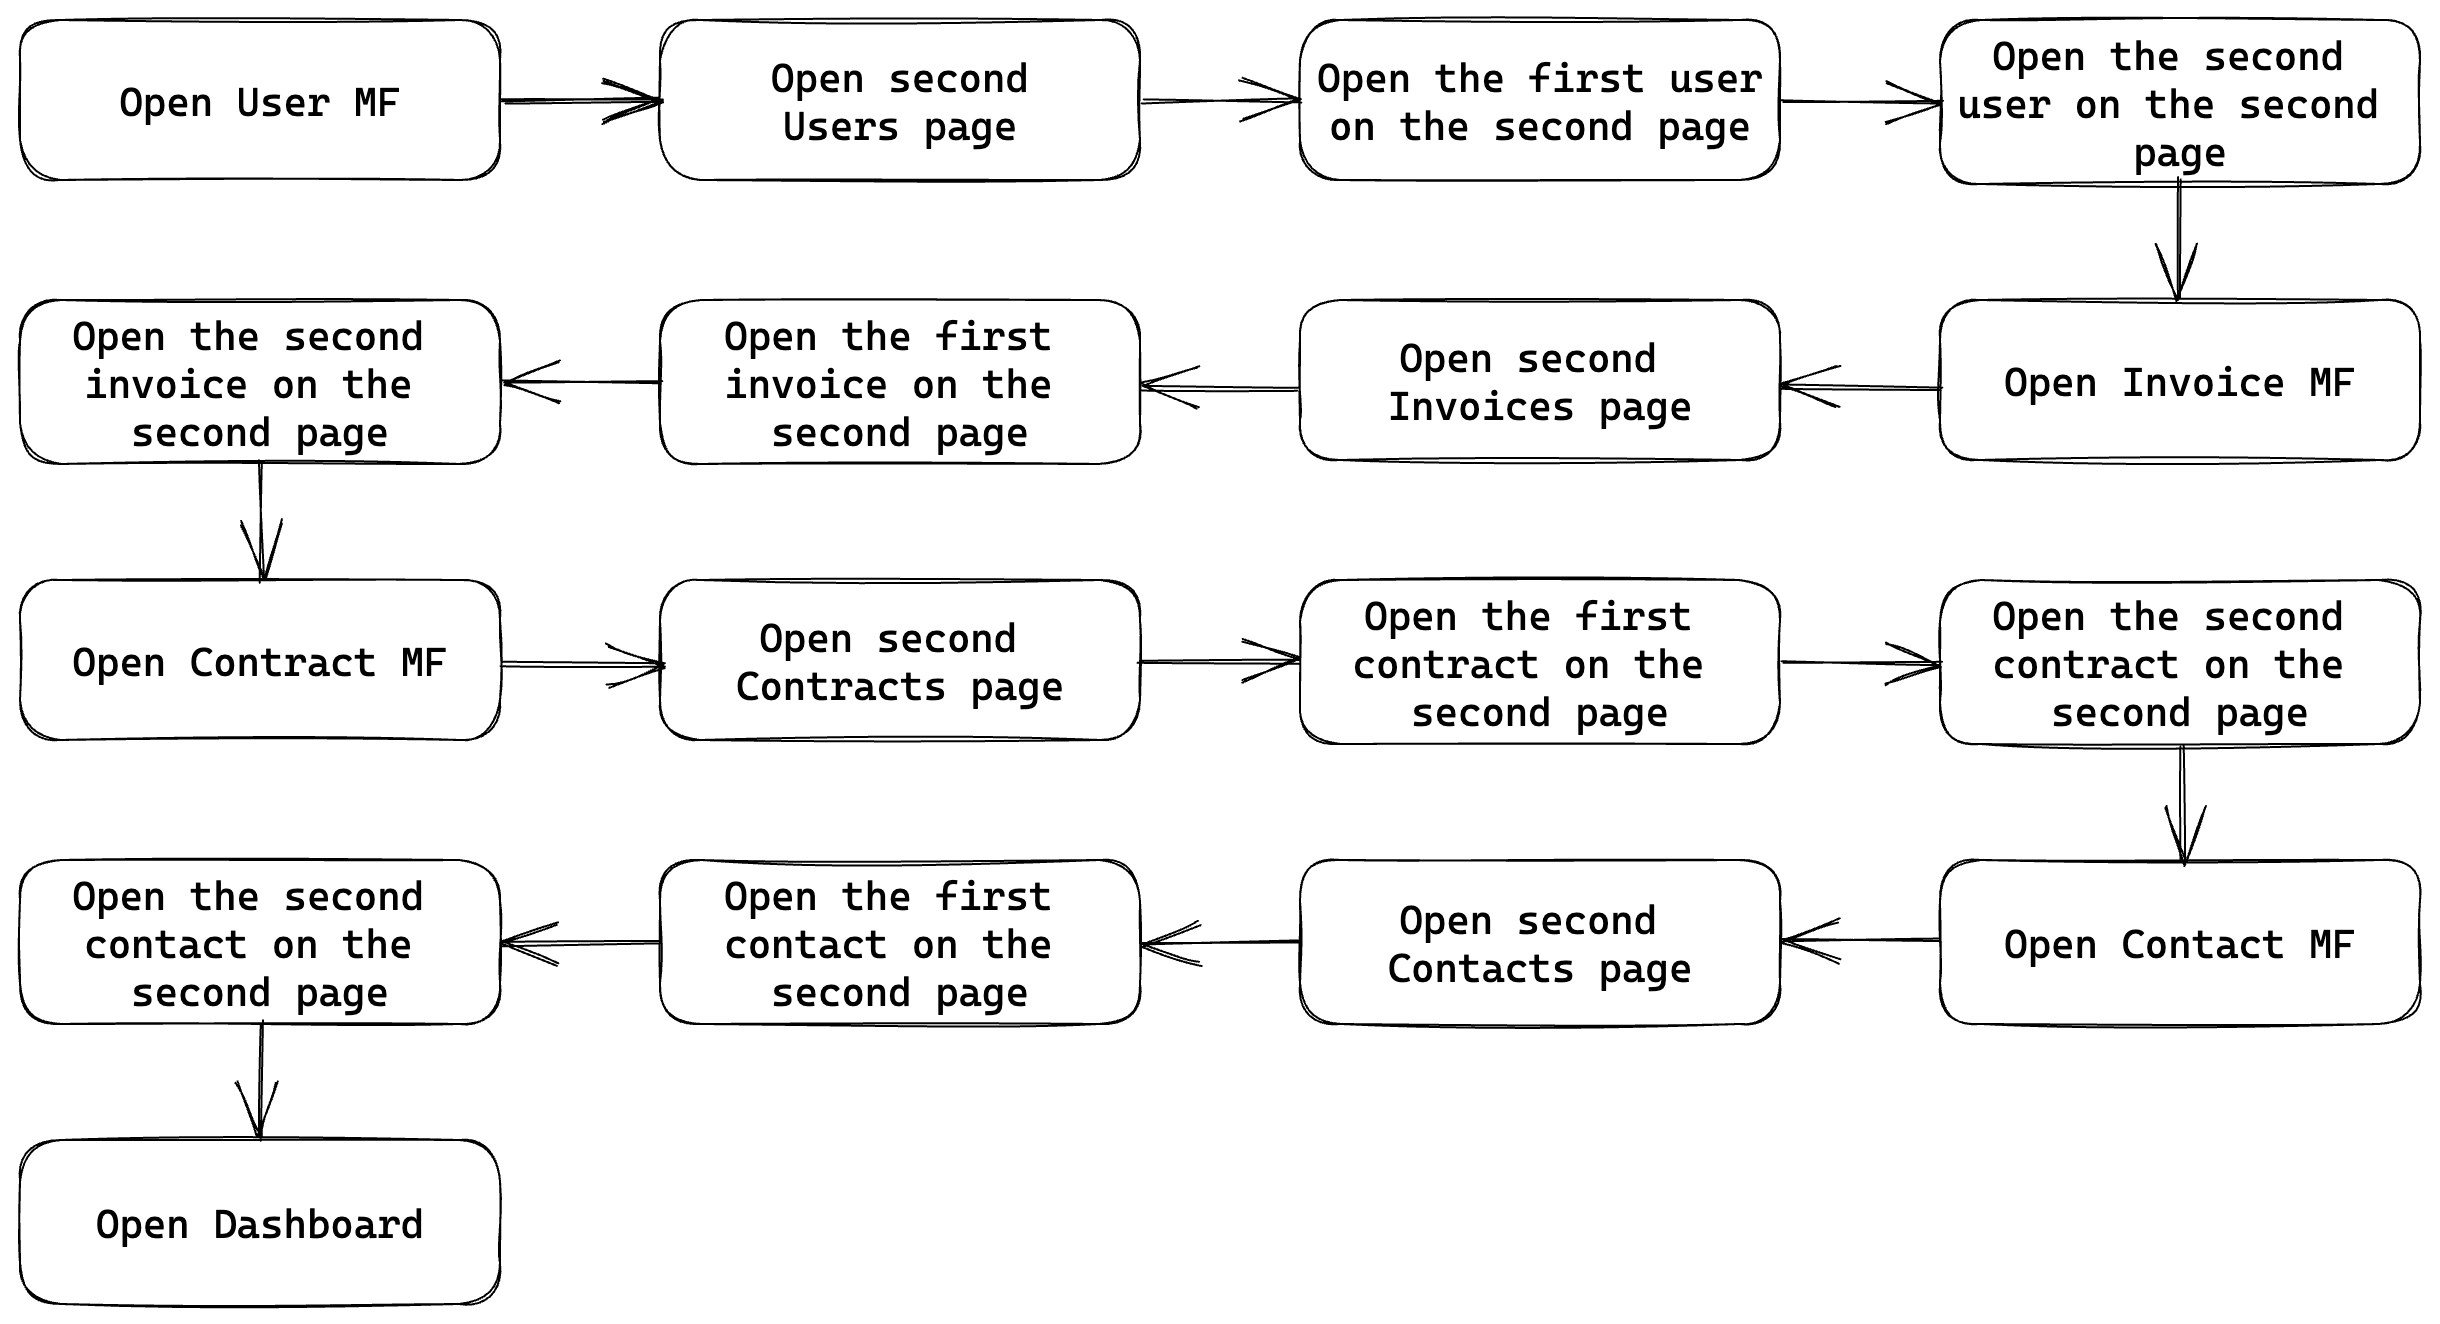
\includegraphics[width=1\linewidth]{images/results/evaluation-second-path.png}
\caption{The second user journey through the application to measure the performance of the micro-frontend architecture.}\label{fig:results:evaluation-second-path}
\end{figure}
\fi

\noindent The following sections compare the three distinct approaches regarding request sizes and response sizes, the number of requests, and the total records fetched, just like in the previous Section \ref{section:results:comparison-first-journey}.

\subsection{Comparing the first- and second-approach}\label{subsection:results:comparison-second-path-first-second-approach}

When comparing the first- with the second approach, there is a difference of 25 network requests made to the GraphQL \ac{API} and the size of the requests and responses, as seen in Table \ref{table:results:size-comparison-second-path-cache-no-reduction-cache-reduction}. No reduced queries are used in this comparison; the 25 extra requests account for the difference in request size and response size. The difference in request size is 26\%, which accounts for about 6.07 KB, which is insignificant. About 22\% of the total response size can be saved by using a shared caching layer. Another interesting observation is that the shared cache approach retrieves 30401 fewer records than the naive approach, about 37\% of the total records returned.

\ifshowTables
\begin{table}[H]
  \begin{tabular}{|l|l|l|l|l|}
  \hline
  & \textbf{Req. size (B)} & \textbf{Resp. size (B)} & \textbf{Requests} & \textbf{Records} \\
  \hline
  \textbf{No Reduction, Separate Cache} & 22955 & 10713304 & 62 & 81325 \\
  \hline
  \textbf{No Reduction, Shared Cache} & 16884 & 8364416 & 37 & 50924 \\
  \hline
  \hline
  \textbf{Diff} & \textbf{6071} & \textbf{2348888} & \textbf{25} & \textbf{30401} \\
  \hline
  \textbf{Reduction (\%)} & \textbf{26\%} & \textbf{22\%} & \textbf{40\%} & \textbf{37\%} \\
  \hline
  \end{tabular}
  \caption{Second Journey: Comparing the requests and responses of the second- and third-approach.}\label{table:results:size-comparison-second-path-cache-no-reduction-cache-reduction}
\end{table}
\fi

\subsection{Comparing the first- and third-approach}\label{subsection:results:comparison-second-path-second-third-approach}

Like the previous comparison, there are again 25 requests less made to the GraphQL \ac{API}. The size of the responses and the requests are similar to the previous section. The results are shown in Table \ref{table:results:size-comparison-second-path-no-cache-no-reduction-cache-reduction}. However, due to the reduction in queries, the difference in the size of the queries and responses is more significant than in Section \ref{subsection:results:comparison-second-path-first-second-approach}. The difference in request size is 36\%, which accounts for 8.24 KB, which is insignificant. A shared caching layer and query reduction can save about 22\% of response size; as before, 37\% fewer records need to be fetched from the \ac{API}.

\ifshowTables
\begin{table}[H]
  \begin{tabular}{|l|l|l|l|l|}
  \hline
  & \textbf{Req. size (B)} & \textbf{Resp. size (B)} & \textbf{Requests} & \textbf{Records} \\
  \hline
  \textbf{No Reduction, Separate Cache} & 22955 & 10713304 & 62 & 81325 \\
  \hline
  \textbf{Reduction, Shared Cache} & 14718 & 8361306 & 37 & 50924 \\
  \hline
  \hline
  \textbf{Diff} & \textbf{8237} & \textbf{2351998} & \textbf{25} & \textbf{30401} \\
  \hline
  \textbf{Reduction (\%)} & \textbf{36\%} & \textbf{22\%} & \textbf{40\%} & \textbf{37\%} \\
  \hline
  \end{tabular}
  \caption{Second Journey: Comparing the requests and responses of the first- and third-approach.}\label{table:results:size-comparison-second-path-no-cache-no-reduction-cache-reduction}
\end{table}
\fi

\subsection{Comparing the second- and third-approach}\label{subsection:results:comparison-second-path-first-third-approach}

Between the second approach and the third approach, there is almost no difference regarding request size and response size. The results are displayed in Table \ref{table:results:size-comparison-second-path-no-cache-no-reduction-cache-no-reduction}. Both approaches have the same number of queries sent to the GraphQL \ac{API} and the same amount of records since all micro-frontends share the same cache instance. The difference in request and response size comes only from using the query reduction mechanism. The difference in request size is 13\%, but they account for just 2.17 KB, which is insignificant. The difference between the response sizes (3.11 KB) is almost zero, like in the first journey.

\ifshowTables
\begin{table}[H]
\begin{tabular}{|l|l|l|l|l|}
  \hline
  & \textbf{Req. size (B)} & \textbf{Resp. size (B)} & \textbf{Requests} & \textbf{Records} \\
  \hline
  \textbf{No Reduction, Shared Cache} & 16884 & 8364416 & 37 & 50924 \\
  \hline
  \textbf{Reduction, Shared Cache} & 14718 & 8361306 & 37 & 50924 \\
  \hline
  \hline
  \textbf{Diff} & \textbf{2166} & \textbf{3110} & \textbf{0} & \textbf{0} \\
  \hline
  \textbf{Reduction (\%)} & \textbf{13\%} & \textbf{0\%} & \textbf{-} & \textbf{-} \\
  \hline
  \end{tabular}
  \caption{Second Journey: Comparing the requests and responses of the first- and second-approach.}\label{table:results:size-comparison-second-path-no-cache-no-reduction-cache-no-reduction}
\end{table}
\fi